\chapter{Project context}

\section{Presentation of the host institute}
\subsection{Presentation of the institute of Algebra}
Algebra (from Arabic: al-dschabr "the joining of broken parts") is one of the oldest scientific disciplines of all. As a doctrine of solving equations and systems of equations, it already developed in Babylon and in ancient Egypt. In the 19th century this theory ("classical algebra") was largely completed by the fundamental theorem of algebra by Gauss and the theorem by Abel-Ruffini. Modern algebra developed - on the basis of the work of Galois and Abel - as the theory of algebraic structures, above all of groups, rings and solids. Algebra has fundamental importance within mathematics, since almost all mathematics is based on sets and operations or relations on their elements. In addition to mathematics, various sub-areas of algebra are essential for other research areas, e.g. for symmetry studies in physics and chemistry or for coding theory and cryptography in computer science.

Algebra is a rich field of science with many exciting and dynamic fields of research.


\subsection{Research interest}
The main research areas at the Institute for Algebra are constraint satisfaction problems, finite group theory, and valued rings and fields. All of these topics require the linking of a variety of mathematical theories such as graph theory, group theory, general algebra, order theory and topology.


\section{Project definition}
\subsection{General frame}
With the major boom in \acrlong{ai}, and especially \acrlong{dl} in the $21^\text{st}$ century. Research institutions are looking for \acrlong{ml} techniques to approximate solutions of hard games that are intractable to humans and even conventional algorithms.

\acrlongpl{mpg} are a class of games on graphs that can be explained very easily\footnote{With a slight modification of rules.} to a layman. In the other hand, it is hard even for computers to guess a good strategy, let alone calculate the optimal one. Therefore, a sophisticated \acrshort{ml} algorithm is needed for that purpose.

\subsection{Motivations}
Recent breakthroughts in \acrlong{rl} techniques made superhuman performances in previously intractable games such as Go \cite{AlphaGo}.
\newline Furthermore, for a popular game like Chess, it even surpassed the strongest conventional engines\footnote{This was at the time of writing the article in \citedate{AlphaZero}. Now, chess engines are a lot stronger, and incorporated \acrshort{dl} methods.} \cite{AlphaZero}. 

This advances were gradually applied to theoretical games such as Stochastic Parity Games \cite{ModelFreeParityGame}.
\newline Now, This interesting, as the class of Stochastic Parity Games is a subclass of \acrfull{smpg}, which is our ultimate goal.

Now, to not dive directly into the stochastic version which is more subtle, we limit our approach to \acrfull{mpg}, but try to make it as general as possible, so that it can be incorporated to the stochastic case. 

\subsection{Presentation of the project}
This work is a different approach for solving \acrshort{mpg}. Exact methods are currently computationally ineffecient, and we will instead opt for approximation methods based on \acrshort{dl}.

In this project, we:
\begin{itemize}
	\item Formalised and analysed  \acrshortpl{mpg}.
	\item Made a Python library for \acrshortpl{mpg} with time-critical functions implemented in C++.
	\item Generated and annotated a large dataset of \acrshortpl{mpg}, using a \acrfull{hpc} system.
	\item Analysed the results, to empirically verify our unproven hypotheses about the game.
	\item Conceptualized and implemented a \acrfull{gnn} model that predicts the optimal strategy for a player.
	\item Implemented a \acrfull{sp} algorithm, based on Alpha Zero \cite{AlphaZero} that uses the \acrshort{gnn} model. 
\end{itemize}, 
\section{Requirement}
\subsection{Functional Requirements}
The ultimate goal of this project is to design and implement a \acrshort{sp} system for \acrshort{mpg}. 

As we were not able to discover any implementation regarding \acrshort{mpg}. Before diving into the modeling part, we implemented and tested a library that we called \textbf{\acrshort{mpg}}. We generated and annotated two large datasets of \acrshortpl{mpg} to understand more properties about the game and strategies. And finally then, we started implementing a \acrshort{gnn} model that will be used as part of the \acrshort{sp} system.

\subsection{Non-functional requirements}
\begin{table}[h]
	\begin{tabularx}{\textwidth}{| p{3cm} | X |}
		\hline
		
		Scope & Requirements  \\
		\hline
		Library & \begin{itemize}
			\item \textbf{Performance}: Time-critical operations should have minimal overhead.
			\item \textbf{Correctness}: The implemented methods must be formally correct.
			\item \textbf{Modularity}: The library should be modular and extensible. 
		\end{itemize}\\
		\hline
		Solver & \begin{itemize}
			\item \textbf{Performance}: Solving a \acrshort{mpg} should take as less time as possible.
			\item \textbf{Robustness}: Each thread should account for a wide range of errors, and resume operation if affected without disrupting the whole program.
		\end{itemize} \\
		\hline
		Analysis & \begin{itemize}
			\item \textbf{Riguour}: The analysis should be as formal as possible, with proofs if possible.
			\item \textbf{Graphical}: The analysis should contain graphical visualisations.
		\end{itemize}\\
		\hline
		Model &\begin{itemize}
			\item \textbf{Dynamic}: The model should work on any graph no matter its size.
			\item \textbf{Symmetry}: The model should account for the symmetries of the game.
			\item \textbf{Stability}: The model's result should only differ slightly when there is a small change in the game parameters.
			\item \textbf{Performance}: The model should not be slower than the conventional solver.
		\end{itemize} \\
		\hline
		Self Play &\begin{itemize}
			\item \textbf{Just in time}: The self play algorithm must support just in time generated graphs.
			\item \textbf{Scalability}: The self playinig system should scale horizontally and vertically.
			\item \textbf{Adaptability}: The system can detect new or defect nodes and act accordingly.
			\item \textbf{Continuity}: The learning process must be 
			\item \textbf{Integration}: The model should account for the symmetries of the game.
		\end{itemize} \\
		
		\hline
	\end{tabularx}
	\caption{Non functional requirements
		\label{table:NonFunctionalRequirements}}
\end{table}
\section{Introduction to Mean Payoff Games}
\subsection{Mean Payoff Games}

\subsection{State of the art}
\acrfull{mpg} are well-known in many fields, such as Optimization \cite{SimplexMPG}, Game Theory \cite{PositionalStrategies}, Formal Verification \cite{OmegaSpecsMPG}, Constraint Satisfaction Problems  \cite{TropicalCSP,MPGMaxAtom}, Reinforcement Learning \cite{StrategyImprovement}.

We believe that \citeauthor{PositionalStrategies} were the first to introduce \acrshort{mpg} in their \citedate{PositionalStrategies} paper \cite{PositionalStrategies} in which they also proved the optimality of positional strategies\footnote{Which will be defined in section \ref{section:Formalisation:Strategy:Positional}}. The problem itself is interesting as it connect many related fields. First of all, it is closely related to many problems in constraint satisfaction \cite{TropicalCSP,MPGMaxAtom}, model-checking \cite{OmegaSpecsMPG}, game theory \cite{PositionalStrategies}.

Also, another interesting fact is that deciding the winner of a mean payoff game is polynomial time equivalent\footnote{Each instance of both problems can be transformed to the other in polynomial time.} to the Max Atom problem \cite{MPGMaxAtom}, which is in $\texttt{NP}\cap \texttt{co-NP},$ but its membership to $\mathtt{P}$ is still open. This is remarkable, there only few problems that share such fate \cite{NPInterCoNP}.


This influenced mainly two research axes. The first deals with solving the decision problem\footnote{The decision problem of a mean payoff game is deciding the winner.}, and the other one deals with the optimization problem\footnote{The optimization problem is calculating the best strategy for each player} related to calculating the optimal strategies. The optimization problem itself can be solved using exact methods \cite{MPGMaxAtom}, as well as iterative methods \cite{StrategyImprovement,SimplexMPG}.

While we did not find a \acrfull{ml} approach on \acrshort{mpg} in the literature, we were able to find some results in a related game, known as stochastic parity games. In fact, a model-free \acrfull{rl} approach was proposed using the Q-learning minimax algorithm \cite{??}. It does only learn specific instances of the game and not a whole family of stochastic parity games.

We were also able to find supervised learning approach on solved instances of that game using \acrfull{gnn} methods. We will base our \acrshort{gnn} algorithms.

\subsection{Potential difficulties}
We believe that our project is 
 
\section{Introduction to learning approaches}
\subsection{Machine learning}
\acrfull{ml} is a subfield of \acrfull{ai}, which is broadly defined as the capability of a machine to imitate intelligent human behavior. \acrshort{ai} systems are used to perform complex tasks in a way that is similar to how humans solve problems.

\acrshort{ml} focalises on the use of data and algorithms to imitate the way that humans learn, gradually improving its accuracy.

To formalise the definition, we will directly use \citeauthor{MachineLearning}'s famous definition \cite[page.~2]{MachineLearning}: \textit{``A computer program is said to learn from experience $E$ with respect to some class of tasks $T$ and performance measure $P$ if its performance at tasks in $T$, as measured by $P$, improves with experience $E$."}

\subsection{Deep learning}
\subsubsection{Neural Networks}
\acrfull{nn}, are a subset of \acrfull{ml} and are at the heart of \acrfull{dl} algorithms. Their name and structure are inspired by the human brain, mimicking the way that biological neurons signal to one another.

\begin{figure}[H]
	\centering
	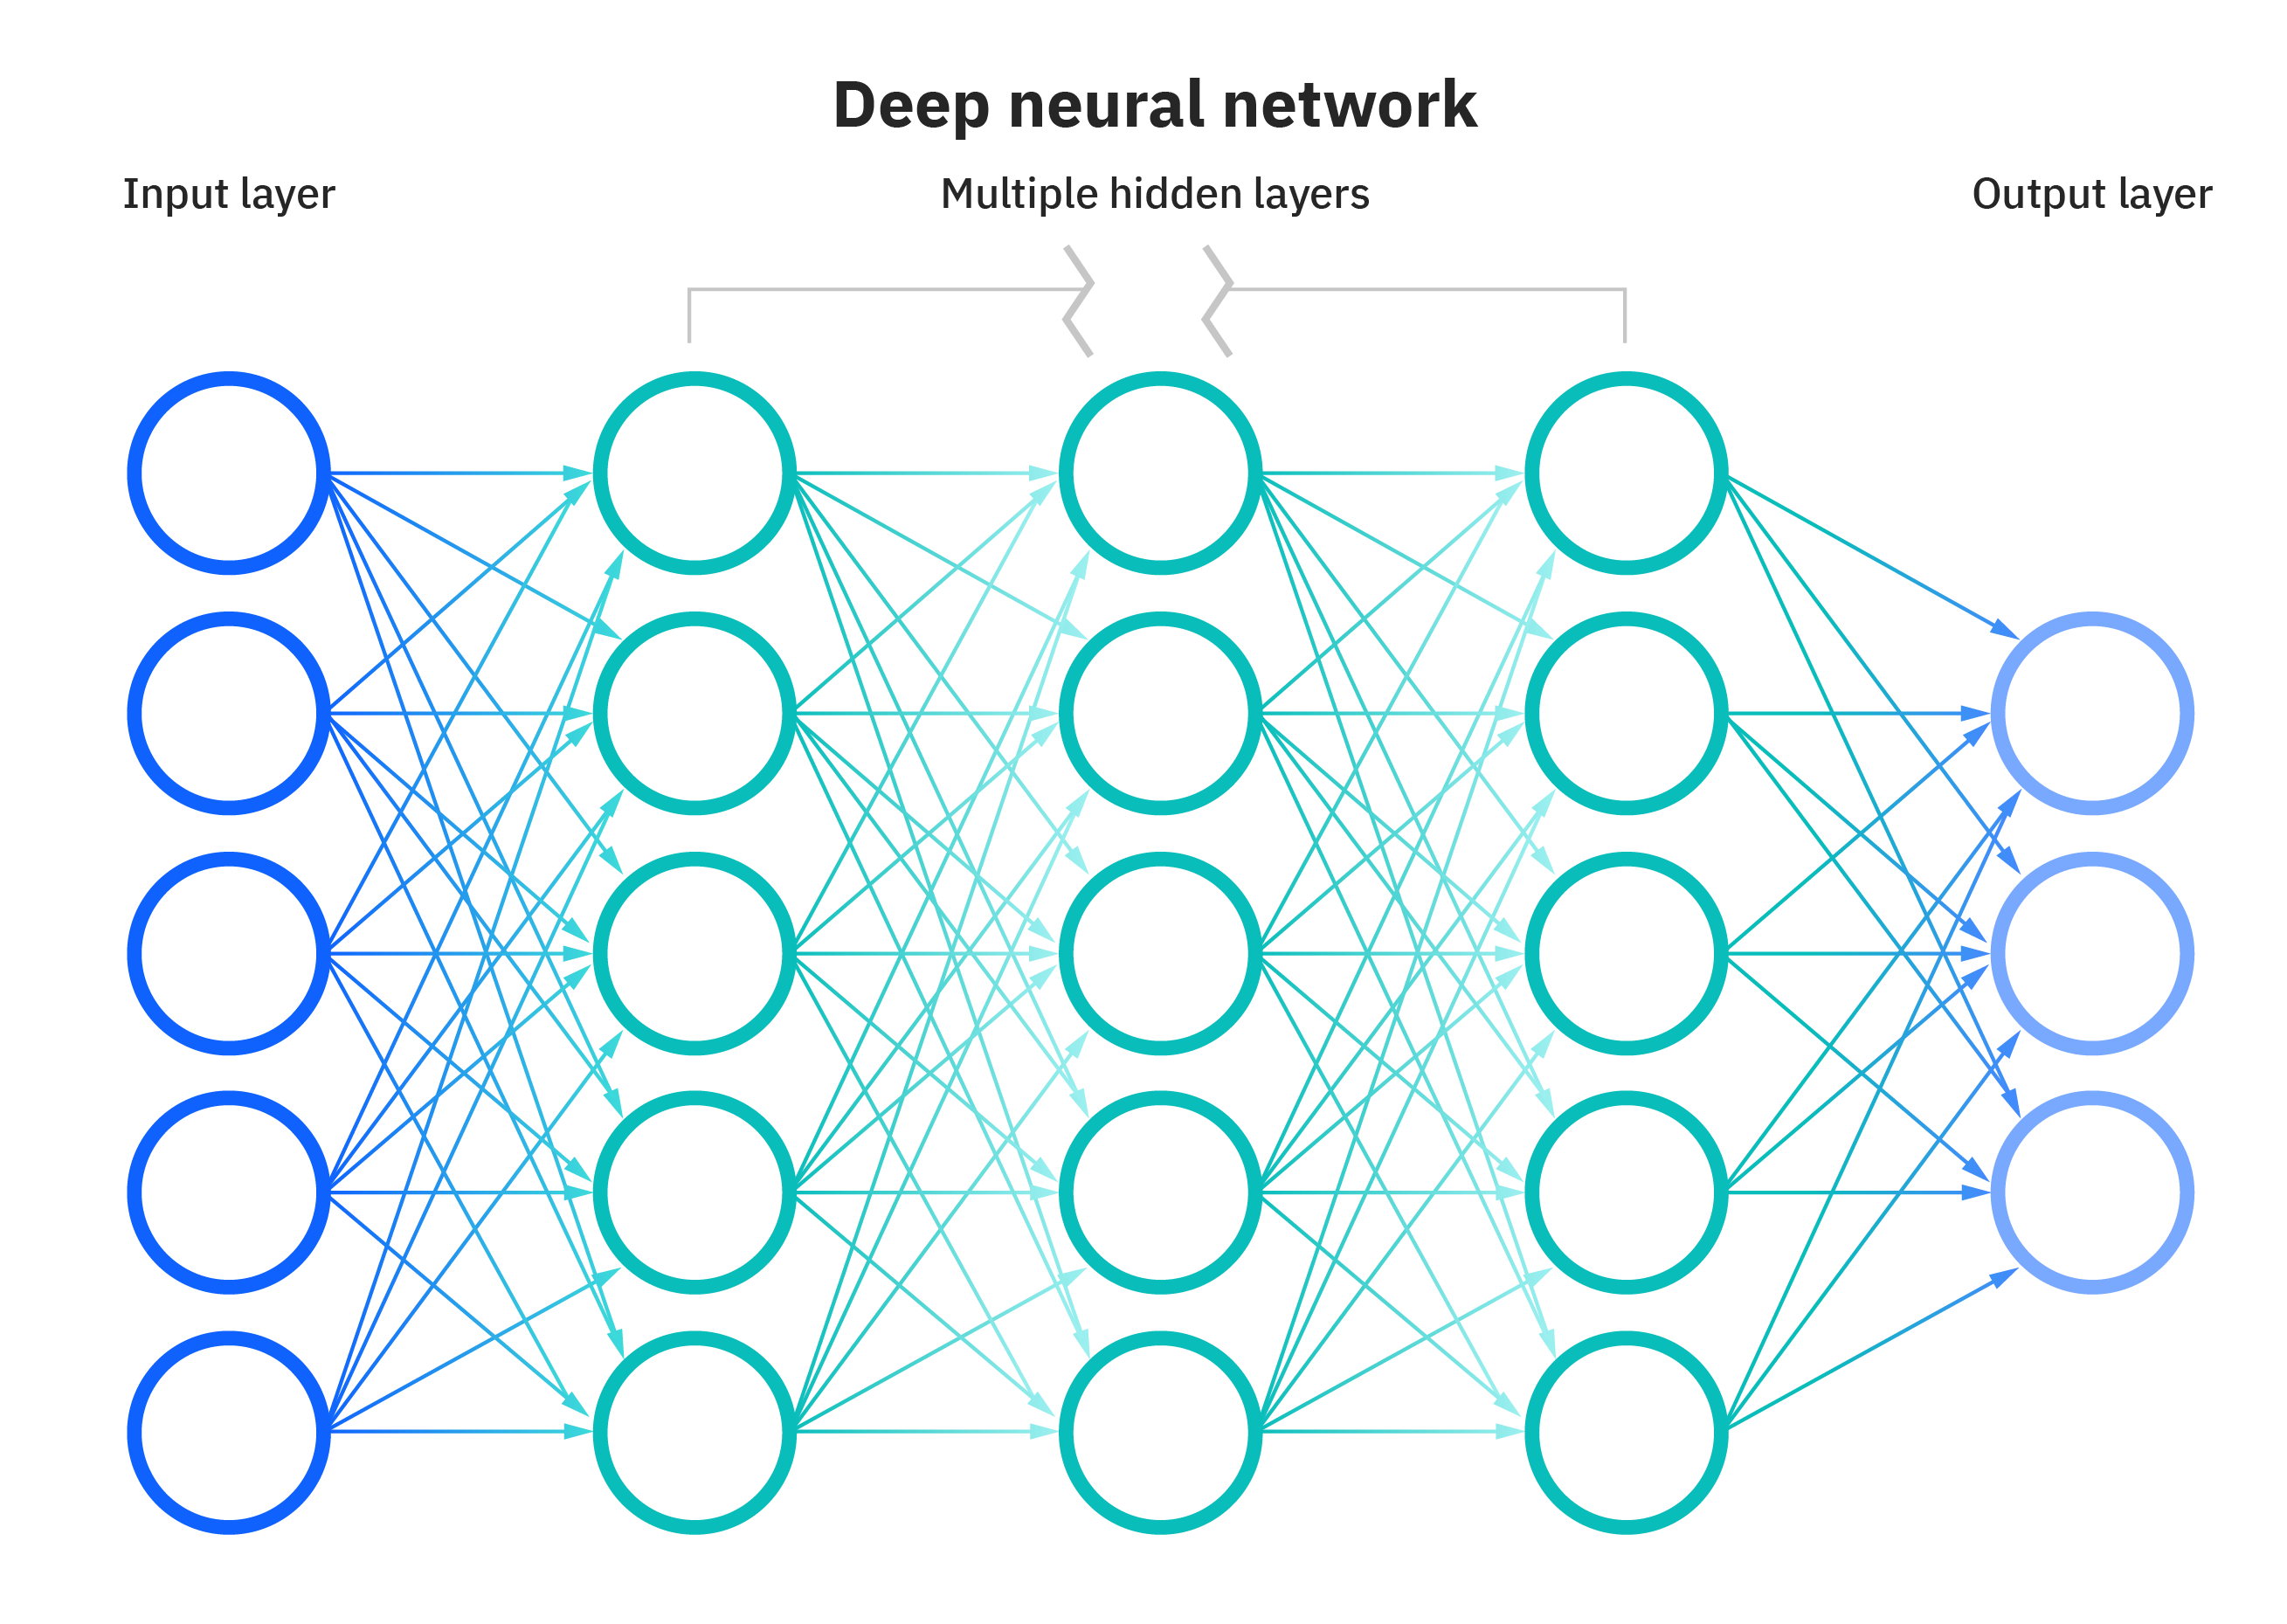
\includegraphics[width=0.75\textwidth]{Figures/NeuralNetwork.png}
	\caption{An illustration of a neural network}
\end{figure}
\FloatBarrier

\acrshort{nn} are comprised of a node layers, containing an input layer, one or more hidden layers, and an output layer. Each node, or artificial neuron, connects to another and has an associated weight and threshold. These series of connections make the possibility to learn complex features from the dataset.

\subsubsection{Definition}
\acrfull{dl} is a subset of \acrfull{ml}, which is essentially a neural network with three or more layers. These neural networks attempt to simulate the behavior of the human brain—albeit far from matching its ability—allowing it to ``learn" from large amounts of data. 

\begin{figure}[H]
	\centering
	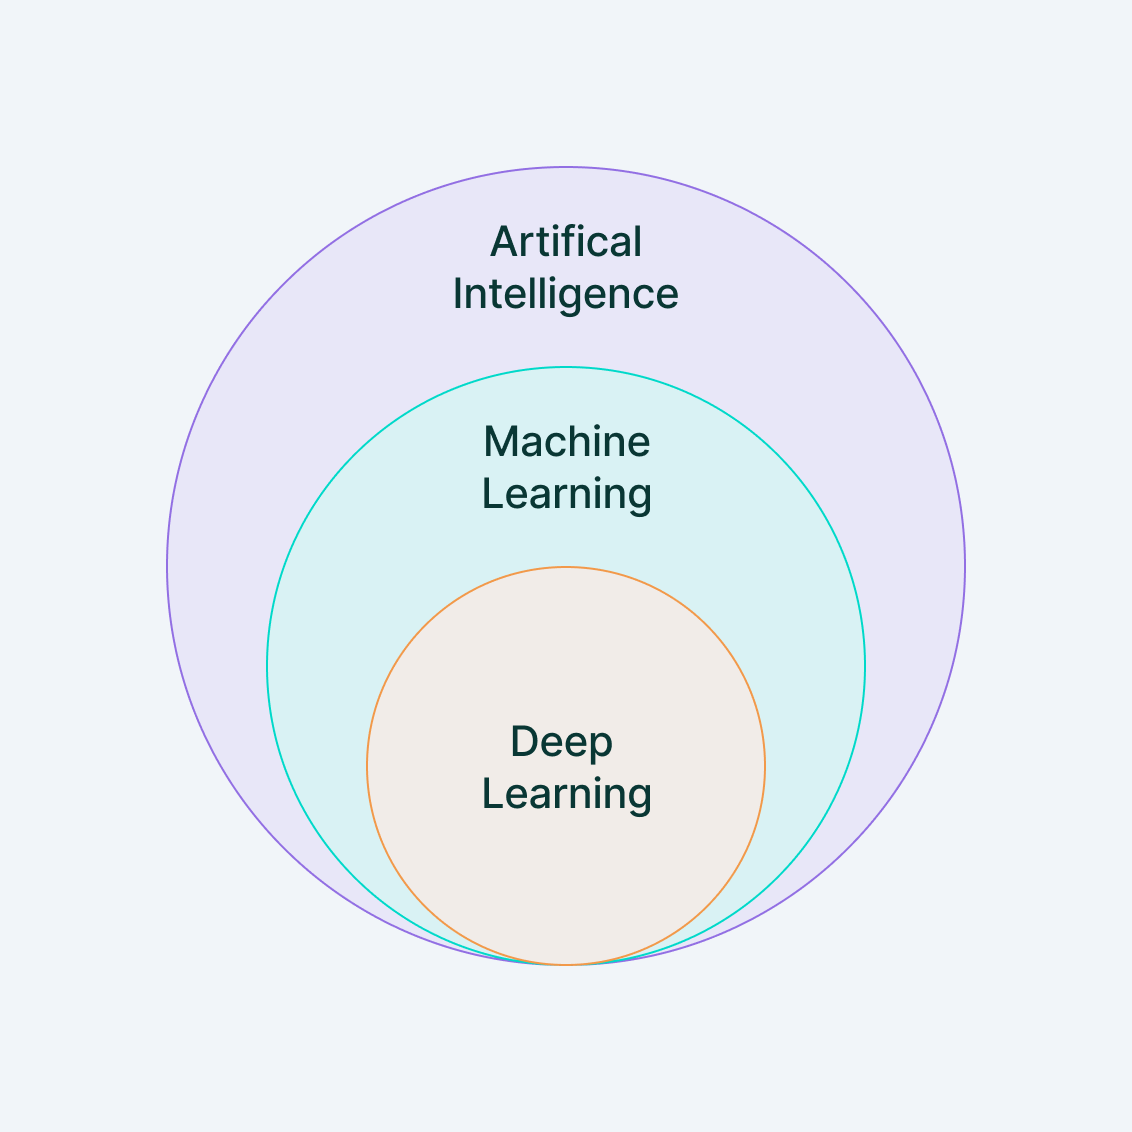
\includegraphics[width=0.5\textwidth]{Figures/AIHierarchy.png}
	\caption{Relation between \acrshort{ai}, \acrshort{ml} and \acrshort{dl}}
\end{figure}
\FloatBarrier

The term deep learning originated from new methods and strategies designed to generate these deep hierarchies of non-linear features by overcoming the problems with vanishing gradients so that we can train architectures with dozens of layers.

\begin{figure}[H]
	\centering
	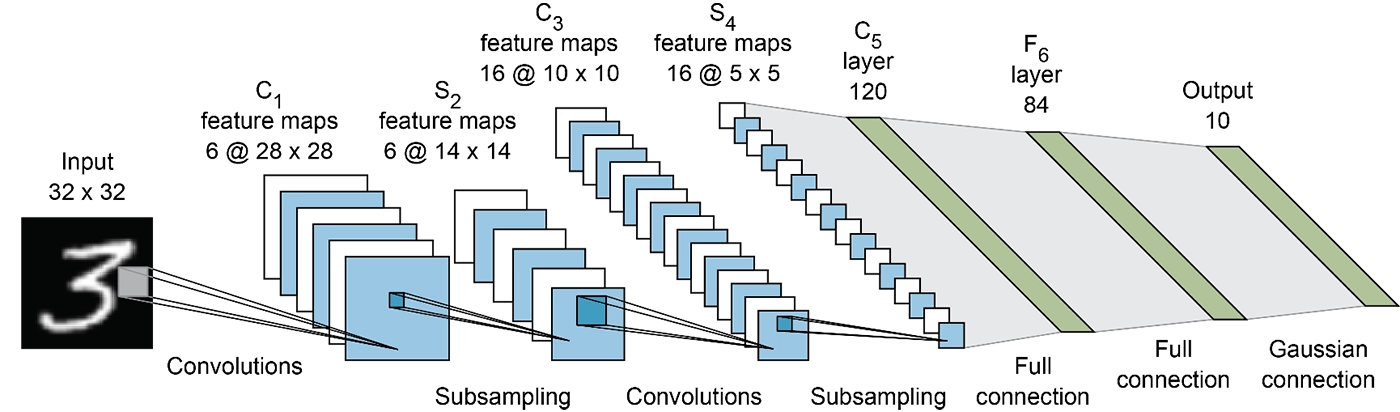
\includegraphics[width=0.75\textwidth]{Figures/CNN.png}
	\caption{An example of deep learning model}
\end{figure}
\FloatBarrier

\subsection{Reinforcement learning}
\acrfull{rl} is the science of decision making. It is about learning the optimal behavior in an environment to obtain maximum reward. This optimal behavior is learned through interactions with the environment and observations of how it responds, similar to children exploring the world around them and learning the actions that help them achieve a goal.

In the absence of a supervisor, the learner must independently discover the sequence of actions that maximize the reward. This discovery process is akin to a trial-and-error search. The quality of actions is measured by not just the immediate reward they return, but also the delayed reward they might fetch. As it can learn the actions that result in eventual success in an unseen environment without the help of a supervisor, reinforcement learning is a very powerful tool.
\begin{figure}[H]
	\centering
	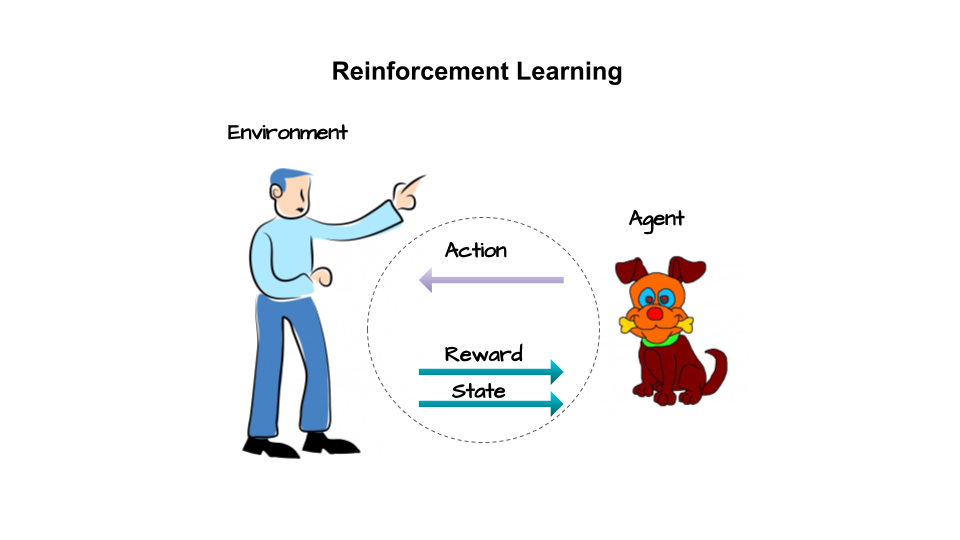
\includegraphics[width=0.75\textwidth]{Figures/RLCartoon.png}
	\caption{An example of a reinforcement learning system}
\end{figure}
\FloatBarrier


Due to its generality, reinforcement learning is studied in many disciplines, such as game theory, control theory, operations research, information theory, simulation-based optimization, multi-agent systems, swarm intelligence, and statistics. 
\subsection{Self Play}
In \acrfull{rl}, the term self-play describes a kind of \acrfull{mal} that
deploys an algorithm against copies of itself to test compatibility in various stochastic environments.

\acrfull{sp} rose to prominence after the great success of Alpha Go \cite{AlphaGo} and its subsequent version Alpha Zero \cite{AlphaZero}.

\begin{figure}[H]
	\centering
	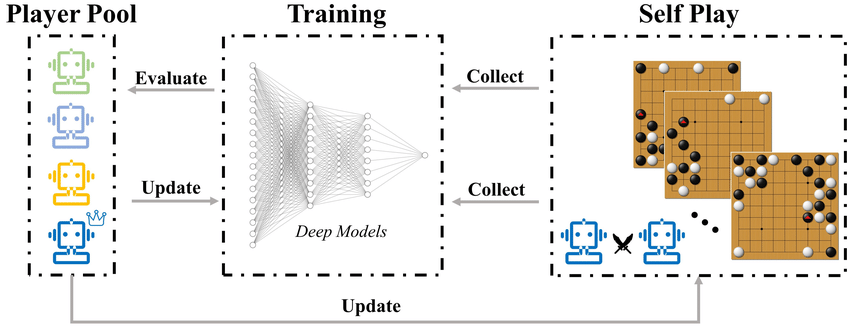
\includegraphics[width=0.75\textwidth]{Figures/AlphaZeroSelfPlay.png}
	\caption{Alpha Go pipeline}
	\scriptsize src: 
\end{figure}
\FloatBarrier

\section{Work methodologies}
This section is dedicated to describing the three methodologies we selected to conduct this
project, complemented by the Gantt chart which illustrates the distribution of our tasks
over the duration of the internship.

Each of the three methodologies we selected dealt with a different part of the project. These parts were very different in nature. As a result, we effectively considered them as distinct subprojects.

The choice of more than one methodology was necessary in our case, as each subproject had to be approached with a unique mindset.

\subsection{Agile Methodology}
As the first goal of the project was to implement and test a \acrshort{mpg} library, we followed the \textbf{Agile} methodology.

\begin{figure}[h]
	\centering
	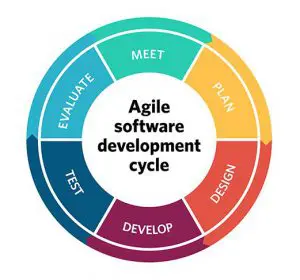
\includegraphics[width=0.4\textwidth]{Figures/Agile.png}
	\caption{Agile development cycle}
\end{figure}
\FloatBarrier

Agile methodology is a project management approach that prioritizes cross-functional collaboration and continuous improvement. It divides projects into smaller phases and guides teams through cycles of planning, execution, and evaluation.

Agile’s entire framework revolves around the program’s core values. Many of the Agile Principles are directly based on these values:
\subsection{Crisp-DM}
The second subproject was to analyse, and implement a reinforcement learning model for \acrshortpl{mpg}. For that part, we used the \textbf{Crisp-DM}

CRISP-DM, which stands for Cross-Industry Standard Process for Data Mining, is an industry-proven way to guide the data mining efforts.

\begin{figure}[h]
	\centering
	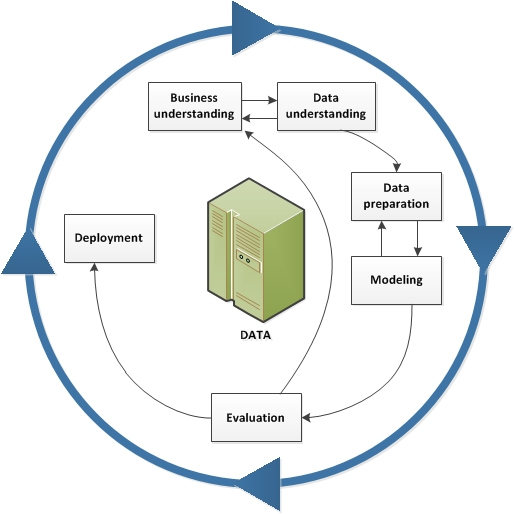
\includegraphics[width=0.5\textwidth]{Figures/CRISP_DM.jpg}
	\caption{Agile development cycle}
\end{figure}
\FloatBarrier

As a methodology, it includes descriptions of the typical phases of a project, the tasks involved with each phase, and an explanation of the relationships between these tasks.
As a process model, CRISP-DM provides an overview of the data mining life cycle.
%Add ,right=0.35
\newgeometry{left=0.35cm,bottom=0.5cm}
\thispagestyle{empty}

\begin{landscape}
	
\begin{figure}
	\noindent
					\vspace*{-2cm}
	\hspace{4.35cm}
		\makebox[\textheight]{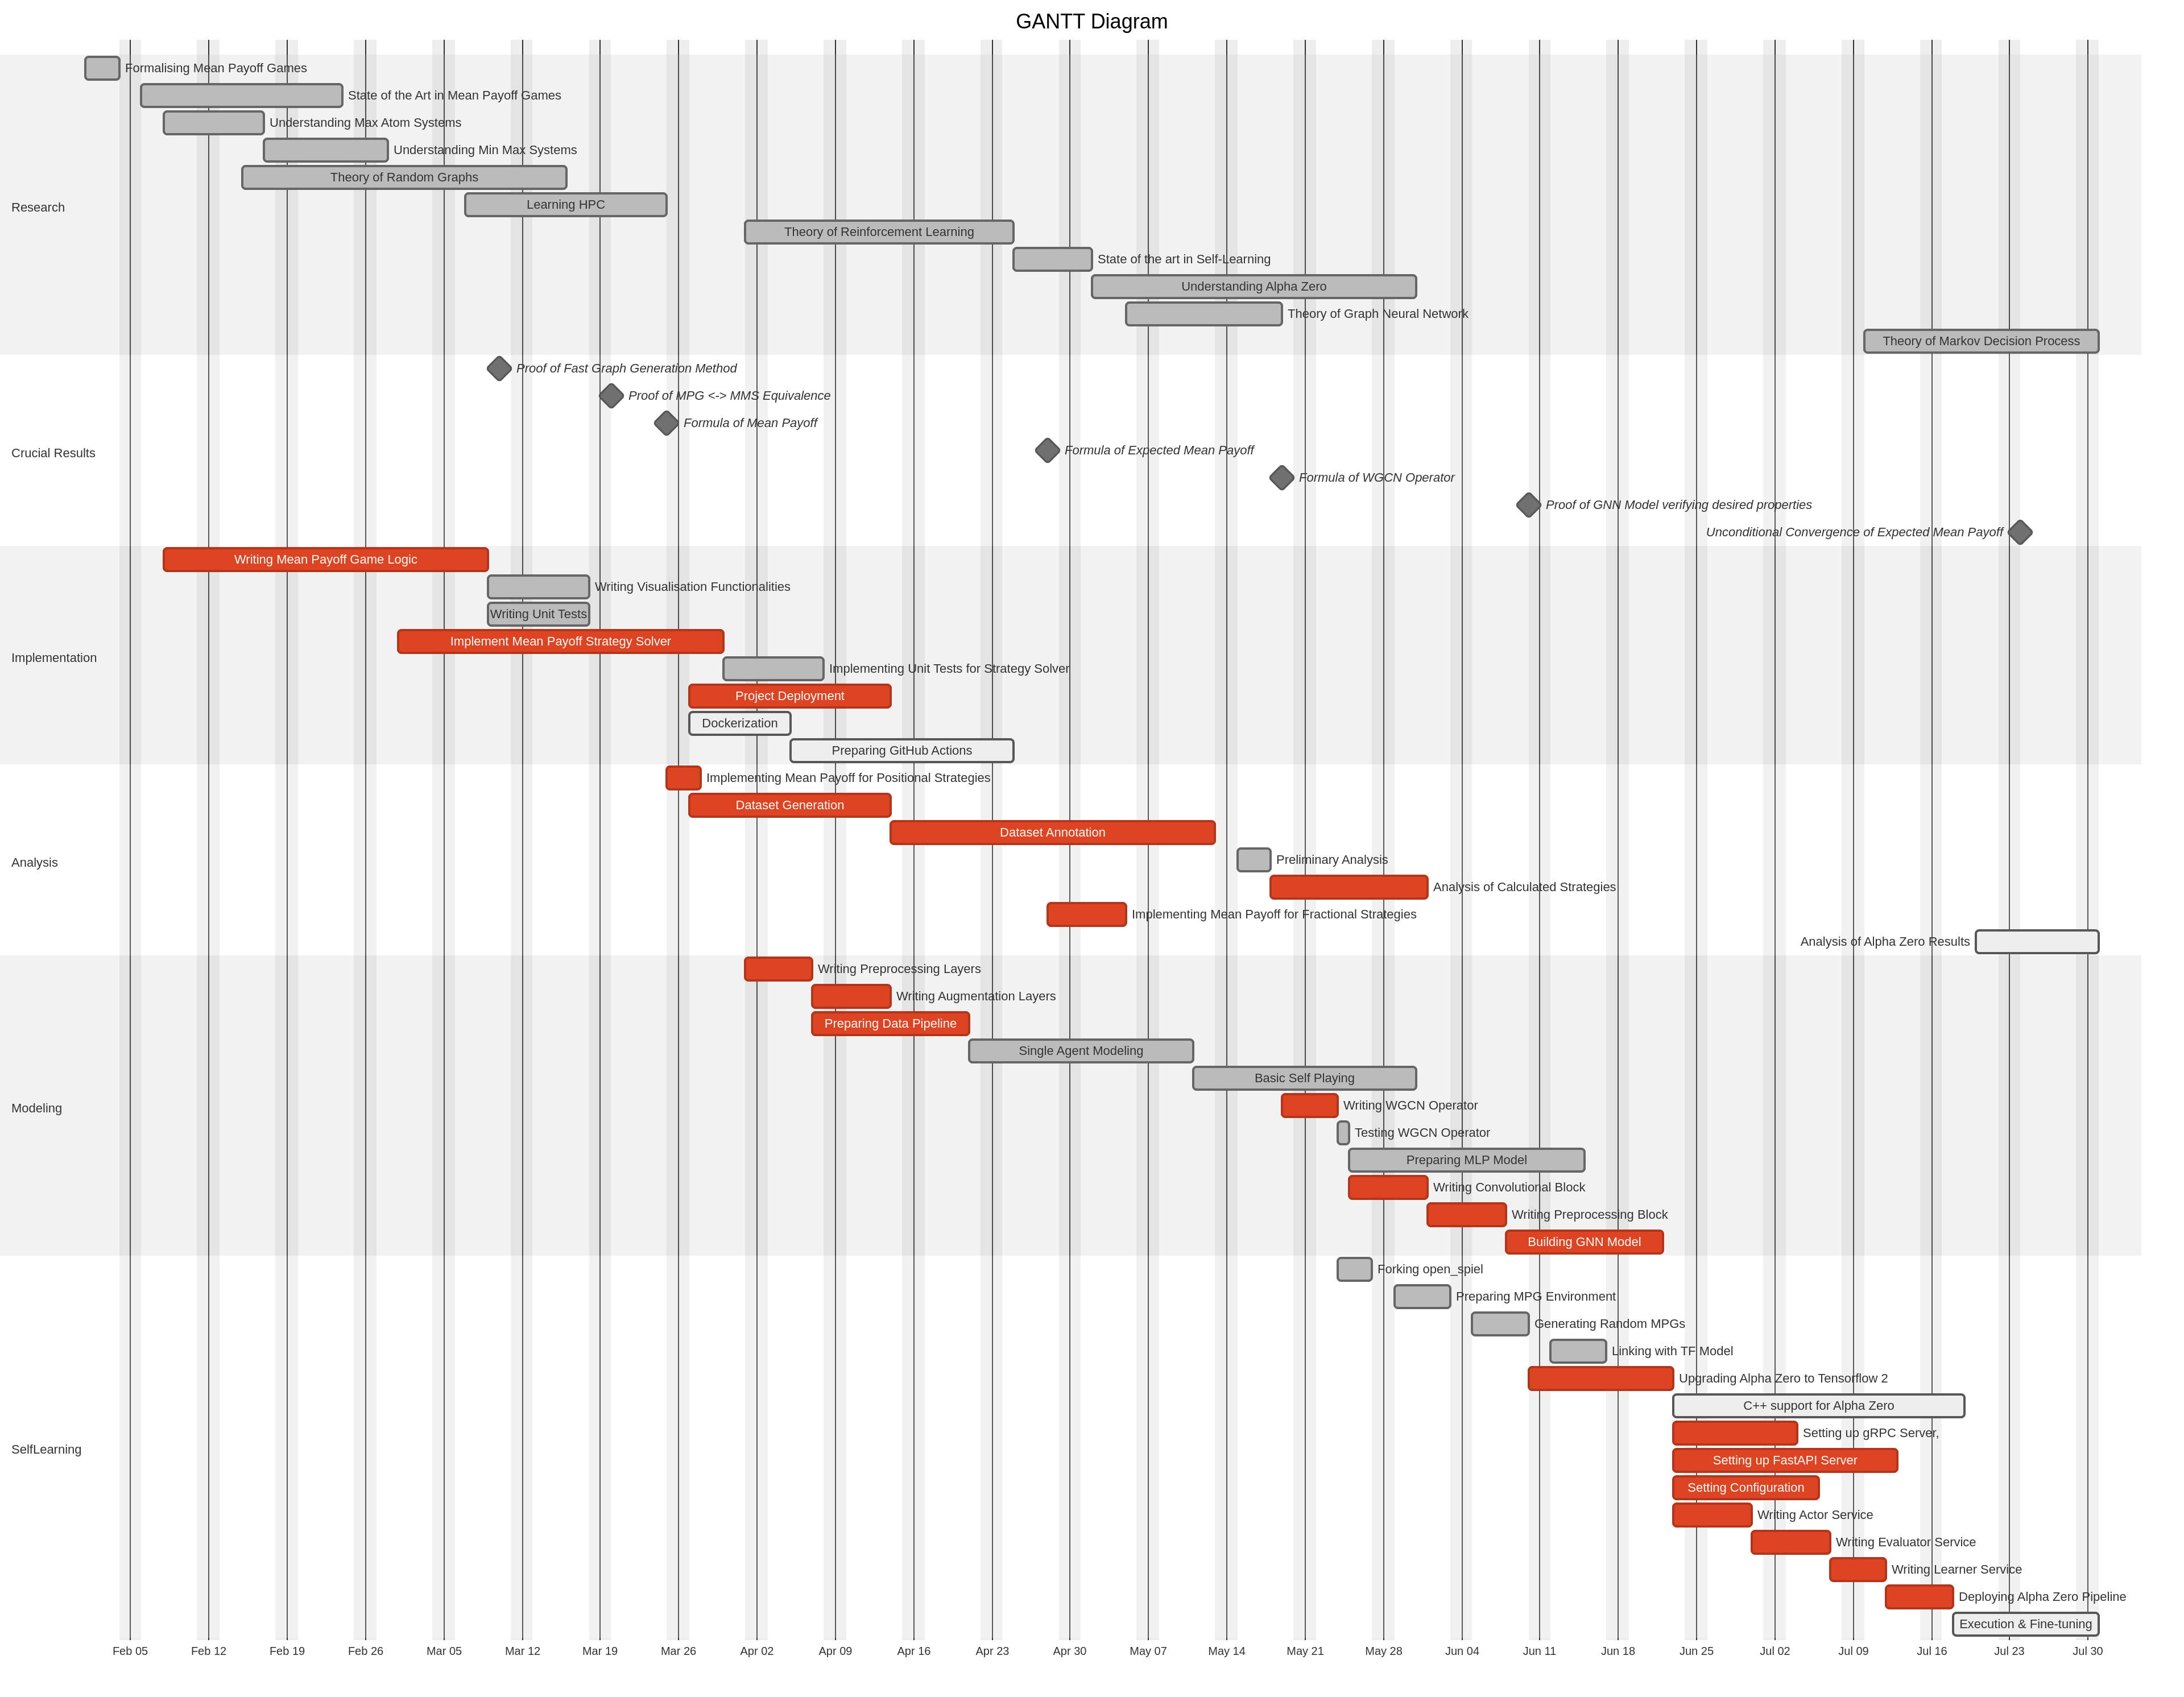
\includegraphics[height=1.2 \textheight]{Figures/Gant.png}}

	\caption{Gantt diagram}

\end{figure}

\end{landscape}
\restoregeometry